\cleartorightpage
%\setcounter{figure}{-1}
%\setcounter{table}{-1}
%\setcounter{section}{-1}
\setcounter{NAT@ctr}{-1}
\chapter*{}\label{chapter:vcap}

\begin{figure}[t!]
\centering

\includegraphics[height=10em]{frontmatter/images/chapter-header-fusion.png}
\end{figure}
\vspace{-4cm}

\phantomsection\addcontentsline{toc}{section}{The Bio: VCaP Chromothripsis}
\articletitle{Gene fusions by chromothripsis of chromo- some 5q in the VCaP prostate cancer cell line}\label{chapter:vcap-paper}

Saskia Hiltemann\textsuperscript{\ref{vcap-affil:emc-bioinf},\ref{vcap-affil:emc-urology},*},
Inês Teles Alves\textsuperscript{\ref{vcap-affil:emc-urology},\ref{vcap-affil:emc-pathology},*},
Thomas Hartjes\textsuperscript{\ref{vcap-affil:emc-urology}},
Peter van der Spek\textsuperscript{\ref{vcap-affil:emc-bioinf}},
Andrew Stubbs\textsuperscript{\ref{vcap-affil:emc-bioinf}},
Jan Trapman\textsuperscript{\ref{vcap-affil:emc-pathology}},
Guido Jenster\textsuperscript{\ref{vcap-affil:emc-urology}}

\small
\begin{enumerate}
\itemsep-0.5em
\item Department of Bioinformatics, Erasmus Medical Center, Rotterdam, The Netherlands.\label{vcap-affil:emc-bioinf}
\item Department of Urology, Josephine Nefkens Institute, Erasmus Medical Center, Rotterdam, The Netherlands.\label{vcap-affil:emc-urology}
\item Department of Pathology, Josephine Nefkens Institute, Erasmus Medical Center, Rotterdam, The Netherlands.\label{vcap-affil:emc-pathology}
\end{enumerate}
\normalsize

\textbf{Published in:} \emph{Human Genetics}, 2013 Jun;132(6):709-13 \\
DOI: \url{https://doi.org/10.1007/s00439-013-1308-1} \\
* Inês Teles Alves and Saskia Hiltemann contributed equally to this work.\\
Supplementary material available online. \\


\section*{Abstract}
The VCaP cell line is widely used in prostate cancer research as it is a unique model to study castrate resistant disease expressing high levels of
the wild type androgen receptor and the \textit{TMPRSS2-ERG} fusion transcript. Using next generation sequencing, we assembled the structural variations in
VCaP genomic DNA and observed a massive number of genomic rearrangements along the q arm of chromosome 5, characteristic of chromothripsis.
Chromothripsis is a recently recognized phenomenon characterized by extensive chromosomal shattering in a single catastrophic event, mainly detected
in cancer cells. Various structural events identified on chromosome 5q of VCaP resulted in gene fusions. Out of the 18 gene fusion candidates tested,
15 were confirmed on genomic level. In our set of gene fusions, only rarely we observe microhomology flanking the breakpoints. On RNA level, only five
transcripts were detected and \textit{NDUFAF2-MAST4} was the only resulting in an in-frame fusion transcript. Our data indicate that although a marker of genomic
instability, chromothripsis might lead to only a limited number of functionally relevant fusion genes.


\section*{Report}
Advances in DNA sequencing technologies have allowed the detailed analysis of genomic aberrations in cancer. Stephens et al. (2011)~\cite{stephens2011massive}, described massive genomic rearrangements, designated ‘chromothripsis’, in a subgroup of chronic lymphocytic leukemia. Subsequently, chromothripsis has been observed in several cancer cell lines, including lung, sarcoma, esophageal, renal, and thyroid cells and in a few patient samples of multiple myeloma, colorectal cancer, medulloblastoma, and neuroblastoma~\cite{magrangeas2011chromothripsis,kloosterman2011chromothripsis,rausch2012genome,molenaar2012sequencing}.

The process of chromothripsis involves the shattering of one or a few chromosomes that is followed by fragment reassembly into derivative chromosomes~\cite{maher2012chromothripsis}. It is defined on the basis of three main features: the occurrence of numerous genomic rearrangements in localized chromosomal
regions; several copy number changes alternating between only one, two, or occasionally three different copy number states; and the alternation between
regions where heterozygosity is preserved with regions displaying loss of heterozygosity~\cite{maher2012chromothripsis}. The localized pattern observed for
chromothripsis differs from that of other types of genomic instability, where rearrangements tend to be dispersed genome-wide~\cite{campbell2008identification,stephens2009complex} and suggests chromothripsis will likely occur when chromosomes are largely condensed. Moreover, the alternation between few copy
number states strongly implies that the chromosomal rearrangements occurred in a short time scale, probably in one single mutational event~\cite{stephens2011massive, righolt2012shattered}.

Several mechanisms have been proposed to induce the massive number of genomic rearrangements observed in chromothripsis. Overall, the clustering
pattern of rearrangements observed in chromothripsis is readily explained by assuming a condensed configuration of the chromosome by the time
chromothripsis was triggered. Moreover, one can also consider, although less reasonably, that a chromosomal region is exposed to localized high-energy
ionizing radiation~\cite{misteli2007beyond}. Along with telomere erosion and breakage–fusion–bridge cycles, also abortive apoptosis after extensive chromosomal
fragmentation and replication stress have been proposed as potential initiating triggers of chromothripsis~\cite{jones2012chromothripsis}.
Currently, the most attractive model for chromothripsis combines both replication stress and mitotic errors with the formation of micronuclei containing
mis-segregated anaphase chromosome(s) that undergo defective DNA replication.

The fragmentation created by this first stage of chromothripsis is further repaired by one of the several DNA repair mechanism~\cite{holland2012chromoanagenesis}.
So far, both non-replicative repair pathways such as non-homologous end joining (NHEJ) and replication-associated repair pathways such as microhomology-mediated
break-induced replication (MMBIR) have been implicated in the reassembly process of pulverized chromosomes~\cite{forment2012chromothripsis}. In case of limited sequence
overlap, non-homologous end joining has been suggested as the most probable molecular mechanism involved in reconnecting the shattered DNA fragments~\cite{rausch2012genome}.
In this study, whole genome paired-end sequencing was performed on DNA from the prostate cancer cell line VCaP~\cite{drmanac2010human}. This cell line is widely
used as a model for research on castration-resistant prostate cancer (CRPC). It is derived from a vertebral metastatic lesion, grows androgen dependently and
has an amplified androgen receptor (AR) gene and the common \textit{TMPRSS2-ERG} fusion gene~\cite{korenchuk2001vcap}. The genome was sequenced at an average coverage
of 113× and an average fully called genome fraction of 97.6 \% (Supplementary methods). Overall, we detected 2,414 high confidence structural variation (SV)
breakpoint events, of which <4 \% juxtaposed portions of gene sequences on both sides (\hyperref[fig:vcap-circos]{Figure~\ref*{fig:vcap-circos}a}). By far, the highest number (573; 24 \%) is
 mapped on chromosome 5q (\hyperref[fig:vcap-circos]{Figure~\ref*{fig:vcap-circos}b}; \href{https://link.springer.com/article/10.1007/s00439-013-1308-1#SupplementaryMaterial}{Table S1}). The remarkable clustering of a massive number of rearrangements on the q arm of chromosome 5 is
a hallmark of the chromothripsis phenomenon~\cite{forment2012chromothripsis}. VCaP has a near-triploid genome, in which most likely the chromothripsis event succeeded
the duplication event. We observe, therefore, a copy number distribution varying mainly between three copy number states and maintenance of heterozygosity
(\hyperref[vcap-gnuplot]{Figure~\ref*{fig:vcap-gnuplot}}, \href{https://link.springer.com/article/10.1007/s00439-013-1308-1#SupplementaryMaterial}{Figure S1}). In addition, the breakpoints in 5q were remarkably clustered in smaller regions with six rearrangements involving a 7-kb
region between 81.121 and 81.128 Mb (\href{https://link.springer.com/article/10.1007/s00439-013-1308-1#SupplementaryMaterial}{Table S1}), although the normal distance between the two joined fragments is normally tens of megabases.

\begin{figure}
    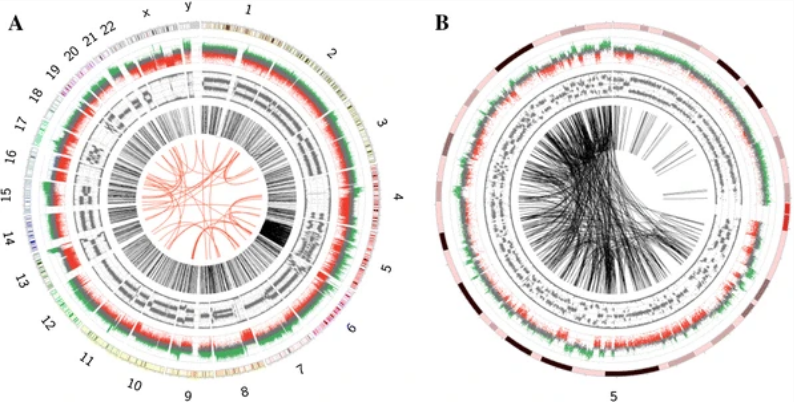
\includegraphics[width=\textwidth]{chapters/images/vcap/circosplots2.png}
    \caption{\textbf{Circos plots showing structural and copy number variation across the whole genome (a) and chromosome 5 (b) of VCaP.} Each chromosome is represented
in the outer ring. The outer data ring corresponds to copy number variation, with regions of gain depicted in green and loss in red. The inner data ring
represents B-allele frequency. The intra and interchromosomal rearrangements are on the inside and depicted in black and red lines, respectively}\label{fig:vcap-circos}
\end{figure}


Out of the 573 SV breakpoints involving 5q, only four were interchromosomal with rearrangements to chromosomes 6 (three events) and 8 (\href{https://link.springer.com/article/10.1007/s00439-013-1308-1#SupplementaryMaterial}{Table S1}). Remarkably,
sequencing of the breakpoint junctions of these SV breakpoints revealed frequent insertions of novel sequences (186/573) (\href{https://link.springer.com/article/10.1007/s00439-013-1308-1#SupplementaryMaterial}{Table S2}). In the gene fusions
resulting from complex chromothripsis rearrangements in 5q, these insertions of up to 255 bp corresponded to fragments of chromosome 5 located within 7–53
Mb distance of the adjacent fusion partner. We rarely observe microhomology flanking the breakpoints in our set of gene fusions, and in a few cases,
we could detect repeats flanking in both sides of the breakpoint junction (\href{https://link.springer.com/article/10.1007/s00439-013-1308-1#SupplementaryMaterial}{Table S3}).


\begin{figure}
    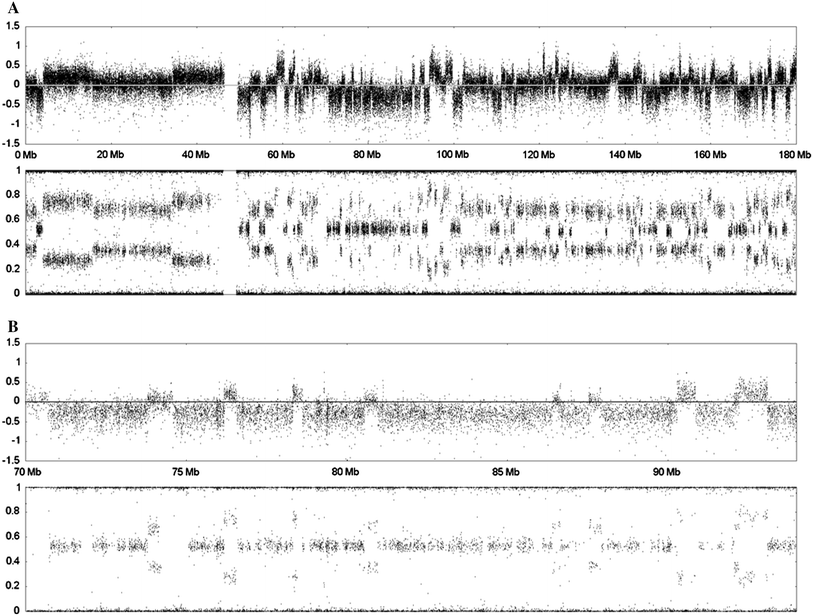
\includegraphics[width=\textwidth]{chapters/images/vcap/gnuplots.png}
    \caption{\textbf{Clustered rearrangements on chromosome 5q of VCaP.} Copy number across chromosome 5 oscillates between a copy number of 2, 3, and 4.
Copy number 2 corresponds to segments of SNP probes below the zero line, copy number 2 to segments of SNP probes in the zero line, and copy number
4 to segments of SNP probes above the zero line. The B-allele frequency plot is displayed below the copy number plot}\label{fig:vcap-gnuplot}
\end{figure}

Forty-three out of the 573 SV breakpoint events on 5q were in different genes at both sides. In 18 of the 43 events, the two different
genes were in the same orientation and potentially encoding a functional fusion protein (\hyperref[table:fusions]{Table~\ref*{table:fusions}}, \href{https://link.springer.com/article/10.1007/s00439-013-1308-1#SupplementaryMaterial}{Figure S2}). In order to validate
the 18 candidate gene fusions on DNA level and check whether the fusion transcripts encode an in-frame fusion protein, we performed
PCR on both DNA and cDNA level. We could validate 15 candidate gene fusions at the DNA level (\href{https://link.springer.com/article/10.1007/s00439-013-1308-1#SupplementaryMaterial}{Figure S3}), whereas only one-third were
detected on mRNA level suggesting downregulation of gene expression or instability of the fusion transcripts~\cite{stephens2011massive}.
Sequencing of the PDE4D-FAM172A breakpoint revealed that within this gene fusion a small fragment of PPP2R2B sequence (55 bp) is inserted
in-between the PDE4D and FAM172A genes. This explains the correct NGS identification of the PDE4D-PPP2R2B and PPP2R2B-FAM172A breakpoints,
 but the absence of a PCR product since the PPP2R2B primers were originally designed outside of the small insert. Conversely, the ADAMTS12-PXDNL
candidate gene fusion had a very low number of discordant mate pairs indicating the fusion event, and hence is most likely a sequencing artifact.
Chromothripsis, being a seemingly random process, results in highly altered chromosomes with numerous mutations and rearrangements. The formation
of gene fusions as a consequence of the chromothripsis event does not seem to be preferential over rearrangements occurring outside genes.
Moreover, we did not observe positive selection for in-frame fusion transcripts, since only one out of the five expressed fusion transcripts
resulted in a feasible fusion protein. The role of this fusion between NDUFAF2 and MAST4 remains to be determined (\href{https://link.springer.com/article/10.1007/s00439-013-1308-1#SupplementaryMaterial}{Figure S4, Table S4}). Using PCR,
we observed that all 15 fusions detected in VCaP were also present in the DuCaP cell line which is derived from a dura mater metastasis from the
same patient that gave rise to VCaP~\cite{lee2001establishment}, indicating that chromothripsis occurred in the cells that resulted in both VCaP and DuCaP
metastases (\href{https://link.springer.com/article/10.1007/s00439-013-1308-1#SupplementaryMaterial}{Figures S3 and S4}) (data not shown). The finding that both VCaP and DuCaP harbor the identical gene rearrangements identified in
chromosome 5 indicates that these were present in the precursor prostate adenocarcinoma lesion and not a cell line cultivation artifact.


\begin{table}[t!]
\begin{tabular}{llllllll}
\toprule
5' Donor&3' Acceptor&Donor&Acceptor&Validated&Validated&In&Discordant\\
gene&gene&Chr&Chr&cDNA&DNA&Frame&mate pairs\\
\midrule
PDE4D & C5orf47 & 5 & 5 & Yes & Yes & No & 218 \\
CPLX2 & UBXD8 & 5 & 5 & No & Yes & No & 55 \\
EBF1 & FBXL17 & 5 & 5 & No & Yes & No & 74 \\
KCNN2 & EBF1 & 5 & 5 & No & Yes & Yes & 509 \\
RASGRF2 & RNF145 & 5 & 5 & No & Yes & No & 71 \\
JMY & DMGDH & 5 & 5 & Yes & Yes & No & 102 \\
TRIM40 & FBXO38 & 6 & 5 & No & Yes & No & 89 \\
LMAN2 & AP3S1 & 5 & 5 & Yes & Yes & No & 191 \\
EFNA5 & PCDHB7 & 5 & 5 & No & Yes & No & 11 \\
YTHDC2 & PPP2R2B & 5 & 5 & No & Yes & No & 8 \\
PDE8B & UIMC1 & 5 & 5 & No & Yes & No & 63 \\
ZFP62 & RGNEF & 5 & 5 & No & Yes & No & 225 \\
NDUFAF2 & MAST4 & 5 & 5 & Yes & Yes & Yes & 197 \\
ADAMTS12 & PXDNL & 8 & 5 & No & No & No & 3 \\
EBF1 & FEM1C & 5 & 5 & No & Yes & No & 11 \\
PDE4D & FAM172A & 5 & 5 & Yes & Yes & No & 119 \\
PDE4D & PPP2R2B & 5 & 5 & No & No* & No & 12 \\
PPP2R2B & FAM172A & 5 & 5 & No & No* & Yes & 7 \\
\toprule
\end{tabular}
\caption{\textbf{List of gene fusions involving chromosome 5 of VCaP.} The column \textit{Donor Gene Chr} refers to the chromosome number of the donor gene, and the column \textit{Acceptor Gene Chr} refers to the chromosome number of the 3' acceptor gene. The column \textit{\# of discordant mate pairs} displays the number of mate pair reads that are discordant in relation to the reference genome build 18 and concordant with the respective reported SV event (gene fusion). The \textit{*} corresponds to by-product events that do not result in a real gene fusion}\label{table:fusions}
\end{table}



In our whole genome study of VCaP cells, we also detected a fairly complex rearrangement involving the TMPRSS2 and ERG genes on chromosome 21q\@.
ehe \textit{TMPRSS2-ERG} fusion in VCaP results from the assembly of the ERG and TMPRSS2 breakpoints with the insertion of two fragments of TMPRSS2 (\href{https://link.springer.com/article/10.1007/s00439-013-1308-1#SupplementaryMaterial}{Table S5}).
This did not disrupt the transcript and open reading frame of the final fusion product~\cite{mertz2007molecular}.

Recently, an association between TP53 mutations and chromothripsis has been observed for acute myeloid leukemia and pediatric
medulloblastoma~\cite{rausch2012genome}. In order to determine the status of TP53 in the VCaP cell line, we examined all the single
nucleotide variants (SNVs) detected by next generation sequencing in the TP53 gene (\href{https://link.springer.com/article/10.1007/s00439-013-1308-1#SupplementaryMaterial}{Table S6}). We observed two homozygous missense
SNVs present in the TP53 coding DNA sequence (CDS): c.742C>T and c.215C>G. The c.742C>T (p.R248 W) is a well-known frequently
observed mutation that fully inactivates TP53. The c.215C>G (p.R72P) is a natural occurring polymorphism in exon 4 of TP53.
As a result of the c.742C>T SNV, the VCaP cell line has no wild type functional p53, a key player in the maintenance of genomic
stability. In addition, we have also examined whether there were SNVs present in DNA repair genes previously shown to be altered
in prostate cancer~\cite{grasso2012mutational} (\href{https://link.springer.com/article/10.1007/s00439-013-1308-1#SupplementaryMaterial}{Table S7}). Interestingly, we found the genes ATM, MLH1, PRKDC, and ERCC5 to have missense
SNVs in their respective CDS\@. The only SNVs described to be mutational were present both in the ATM gene (COSMIC mutation ID number
21826 and 21827), but the functional relevance of these remains unknown~\cite{gumy2006atm}. An SNV present in the intron 7
acceptor splicing site of the XRCC4 gene (rs1805377) has shown to be significantly associated with increased prostate cancer risk~\cite{mandal2011polymorphisms}. The homozygous missense c.655A>G SNV present in the MLH1 gene (p.I219V) has been associated with increased
risk of colorectal cancer~\cite{campbell2009mismatch}. Deficiencies in the DNA mismatch repair system are commonly observed in colorectal
cancer and to a less extend in prostate cancer. The influence of the c.655A>G (p.I219V) missense SNV in the development of prostate
cancer remains undetermined.

Here, we report the structural variations detected in VCaP and show that the q arm of chromosome 5 has undergone chromothripsis.
Chromosome 5 appears to be frequently affected by chromothripsis with studies showing the same pattern in a renal cancer cell line~\cite{stephens2011massive} and a neuroblastoma patient~\cite{molenaar2012sequencing}. It remains undetermined, however, whether chromosome-specific
properties or the nonrandom radial localization of chromosomes in distinct territories play a role in the preferential target of certain
chromosomes by chromothripsis. Whether the catastrophic events on 5q in VCaP and the related cell line DuCaP have been playing and still
playing an important role in tumorigenesis remains to be determined.

The massive number of genomic breaks occurring in chromosome 5q hampers the formulation of a definitive model for the generation of chromothripsis.
The copy number variation and B-allele frequency of chromosome 5q in VCaP is a repetition of regions with n2 (AB), n3 (AAB), and n4 (AAAB) (\href{https://link.springer.com/article/10.1007/s00439-013-1308-1#SupplementaryMaterial}{Figure S1}).
Based on chromosome painting, VCaP is an overall near-triploid cell line with four copies of chromosome 5 that vary in size (~68–74(3n), XXYY)
(van Bokhoven et al. 2003). We hypothesize that this pattern is explained by two normal chromosome copies (n2 (AB)) and two copies of A with
chromothripsis (n4 (A*A*AB)), of which one of the two copies has undergone additional rearrangements resulting in n3 (A*AB). The sequence of
events that would lead to this pattern is a duplication of A and B (AABB) and subsequent loss of one B-allele (AAB). One of the A-alleles would
have undergone chromothripsis (A*AB) and duplication (A*A*AB). Additional rearrangements (deletions or even a second chromothripsis event) would
explain the observed 5q regions of n3 (A*AB) (\href{https://link.springer.com/article/10.1007/s00439-013-1308-1#SupplementaryMaterial}{Figure S5}). Our study has shown that research on genes located on and transcripts derived from
chromosome 5q need to take the chromothripsis into account. Besides, being a widely used model for research on AR, ERG, and CRPC, VCaP might
prove a highly relevant model for research on chromothripsis.

\section*{Acknowledgements}
This study was supported by the Complete Genomics Inc.\ grant (EMC GL 083111), the FP7 Marie Curie Initial Training Network PRO-NEST
(grant number 238278) and the CTMM (Center for Translational Molecular Medicine) Translational Research IT (TraIT).

%\includepdf[pages=1-5]{chapters/myarticles/VCaP.pdf}

\footnotesize
\bibliographystyle{ieeetr}
\bibliography{references}
\normalsize
